\chapter{Alternatives to Dark Matter}
\label{sec:MOND}
 
As reviewed in chapter~\ref{sec:evidences}, observations of a wide range of systems at vastly different scales provide compelling evidence for a discrepancy between the visible and inferred masses of these systems. Much of our discussion has centered on interpreting this discrepancy through the lens of an additional substance known as Dark Matter. In this final chapter we revisit these observations to discuss how and to what extent they can be understood through alternative interpretations that do not involve the introduction of extra matter.

The present puzzling mystery of the missing mass has some similarities to the one that the astronomy community was facing in the 1840s: the orbit of the planet Uranus, at the time the farthest known  planet in the solar system, had been observed to violate the standard Newtonian laws of celestial mechanics. 
This led 
the french astronomer Urbain Le Verrier
to postulate the existence of an extra planet whose gravitational effect would explain the anomalies in Uranus's behavior.\footnote{Independently, 
John Adams, working at Cambridge in England, put forward the same idea, but his works were not published until later.}
Such a planet, named Neptune, was indeed observed in 1846 by 
Johann Galle, 
almost exactly at the position indicated by Le Verrier on the basis of his computations~\cite{Neptune}.
During the same period, an additional anomaly was being discussed in the astronomy community: the planet Mercury was also displaying a puzzling feature not predicted by the Newtonian gravity --- the precession of its perihelion. This led once again Le Verrier to interpret the observed deviation as the gravitational effect of yet another hypothetical planet, which was named Vulcain. 
Despite decades of searches and even some false discoveries, Vulcain was never found.
Instead, this anomaly indicated new physics beyond the paradigm of the time:
the anomaly was later understood by Albert Einstein as a correction to Newtonian gravity due to General Relativity~\cite{Vulcain}.

\smallskip

The analogy with the topic of this review is evident: we are now in a similar situation since we only have indirect gravitational `anomalies'.
Are they due to some extra (dark) matter, as was the case for Neptune, or are they due to extra gravitational physics, as in the case of the non-existent Vulcain? So far, no convincing modification of gravity has been proposed which can reproduce all the anomalies described above. Hence, most of the community currently directs its efforts toward the first possibility, i.e., that there is additional matter.
Nevertheless, DM has never been observed directly.
Interesting alternative ideas have been proposed that can fit a sub-set of the gravitational anomalies. Below, we review these ideas.







\section{Puzzling regularities in galactic rotation curves}\index{Rotation curves}
Attempts to propose alternative ideas to DM started already early on, when galactic rotation curves were 
the main evidence for DM (a role played today by the formation of structures in cosmology).
Galaxies are now regarded as complicated but ordinary objects, 
and thereby as unlikely places where new fundamental physics might show up.
More technically,
attempts to explain galactic rotation curves through unusual modifications of gravitational dynamics generically fail when one adds new dependencies on size, density or curvature. This is because galaxies are not extreme objects in terms of these variables, hence modifications of General Relativity in galactic conditions typically lead to larger deviations elsewhere, in disagreement with observations.
However, galaxies probe extremely small accelerations, 
opening the door for a modified dynamics in this regime.

\subsection{Rotation velocities at asymptotically large radius}\index{Rotation curves!flatness}\index{MOND!rotation curves}
The first intriguing observation in this sense was that rotation curves 
asymptotically tend to a constant rotation velocity $v_\infty$.
In the context of DM this regularity is understood to be due to the specific form of the density profile $\rho(r)$, that is
produced by self-similar collapses, as discussed in section~\ref{sec:rho_from_obs}.
Alternatively, this regularity was interpreted by M.~Milgrom as a new physical law
known as the Modified Newtonian dynamics (MOND)~\cite{MOND}.
MOND postulates that below some critical acceleration $a_*$  the usual Newton law $F=ma$ 
changes to $F=ma^2/a_*$,
where the quadratic dependence 
has been chosen such that the rotation curves become flat at accelerations below $a_*$.
Using $a=v^2/r$ and spherical approximation, gives the scaling behaviours
\beq 
\bbox{\frac{Gm{\cal M}_b(r)}{r^2}=
F \simeq \left\{ \begin{array}{ll}
ma &  a \gg  a_*,
\cr
ma^2/a_* &  a \ll a_*,\end{array}\right.}
\quad \Rightarrow\quad
v(r)\simeq \left\{
\begin{array}{ll}
(G{\cal M}_b(r)/r)^{1/2} & \hbox{Newton},\cr
(G{\cal M}_b(r)a_*)^{1/4} & \hbox{MOND},
\end{array}\right.
\label{eq:MOND}
\eeq
where ${\cal M}_b(r)$ is the {\em baryonic} mass inside a sphere of radius $r$.
There is no DM in this interpretation.
More formally, the flatness of rotation curves arises because
the modified Newtonian dynamics $a^2 \propto 1/r^2$ is invariant under dilatations of
space and time.



\begin{figure}[t]
\begin{center}
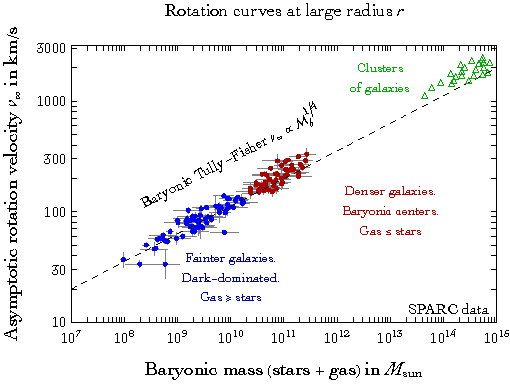
\includegraphics[width=0.6\textwidth]{figs/BaryonicTullyFisherPlot2} \end{center}
\caption[Tully-Fisher]{\em\label{fig:MONDdata}
{\bfseries Baryonic Tully-Fisher} correlation $v_\infty\propto {\cal M}^{1/4}_b$
 among galactic baryonic mass ${\cal M}_b$ and rotation velocity $v(r)$ at asymptotically large radii $r$.
Galaxies with larger (smaller) surface brightness are in red (blue).
(\href{http://astroweb.cwru.edu/SPARC}{\color{black}SPARC galaxy data} from 
\arxivref{1901.05966}{Lelli et al.~(2019)}  in~\cite{Tully-Fisher};
cluster data from \arxivref{0707.3795}{McGaugh (2007)} in~\cite{gobsgbar}).}
\end{figure}


The above eq.\eq{MOND} implied that the asymptotic rotation velocities at large $r$
should scale as a well-defined power of the galactic mass
\beq v_\infty \propto {\cal M}_b^{1/4} .
\label{eq:BTF}\eeq
The observational verification of this expression is known as the {\em baryonic Tully-Fisher relation}\footnote{The earlier Tully-Fisher relation, $L\propto v_\infty^4$, is an approximate empirical  correlation
 between the intrinsic total luminosity of the galaxy, $L$, and the rotational velocities, $v$, on the outskirts of spiral galaxies. 
The proportionality constant is found to be nearly universal, independent of the type and the size of the galaxy. The luminosity $L$ is a measure of the total {\it stellar} mass in the galaxy. Summing the stellar mass and the matter in the form of gas, gives instead the total {\it baryonic} mass ${\cal M}$ in the galaxy. The {\it baryonic} Tully-Fisher relation, ${\cal M}_b \propto v_\infty^4$, has a smaller observational scatter in the values of the proportionality constant for different galaxies than does the scatter in the Tully-Fisher relation $L\propto v_\infty^4$.}~\cite{Tully-Fisher}. 
The rotation curves have now been observed for about 200 galaxies, spanning
about 4 orders of magnitude in $ {\cal M}_b$:
the data plotted in fig.\fig{MONDdata} are compatible with the universal law given in eq.\eq{BTF}.
The scatter around this prediction could well be due to experimental uncertainties, 
which are significant and can reach up to about a factor of 2.

In view of the significant diversity among galaxies, one could have expected a wider distribution.
The heavier galaxies (plotted in red) have high surface brightness:
their center contains a high density of baryonic stars,
so that the rotation curves rise steeply up to the particular asymptotic  constant  value of $v$.
The lighter galaxies (plotted in blue) have low surface brightness:
their baryonic content is mostly in the form of a diffuse gas, and their rotation curves rise slowly.
This can be seen from the rotation curves plotted in the center-right panel of fig.\fig{rotationcurves}.
Example of each of the two types of galaxies are also plotted in more detail in
the bottom row in fig.\fig{rotationcurves}
(see also fig.~2 in \arxivref{astro-ph/9801123}{McGaugh \& de Blok (1998)} in~\cite{DMvsa0}).
The brighter galaxies have baryon-dominated centers, while the fainter galaxies are dominated by a dark component.
Despite the differences, observations found that the fainter 
dwarf galaxies also follow the Tully-Fisher relation. 
This gave MOND a large boost in interest, and
is arguably the most important successful prediction from MOND.

\smallskip

Independently from MOND, the observed baryonic Tully-Fisher relation means that
the galactic rotation curves 
tend to flatten to a constant velocity
at large radii,
when the acceleration $a $ falls below the {\em common critical value}
\beq  \label{eq:aMOND}
\bbox{a_* \approx (1.2\pm 0.1)\, 10^{-10}\, {\rm m}/{\rm s}^2}~,
\eeq
numerically close, in natural units, to the present Hubble constant and to the inverse age of the Universe 
$H_0 \simeq 67.4 \,{\rm km/(s}\cdot{\rm Mpc)} \simeq 6.5~10^{-10} \, {\rm m/s}^2   \sim 1/T_{\rm U}$.
The above critical acceleration is common to almost all galaxies, 
even though galaxies have different sizes and masses.
Equivalently,  a common $a \approx G {\cal M}_b/r^2$ means that smaller galaxies have lower
densities $\rho \propto {\cal M}_b^{1/2}$, which is
also plotted as the correlation ``$\hbox{mass}\propto \hbox{size}^2$'' in the catalogue in fig.\fig{catalogue}.



\begin{figure}[t]
\begin{center}
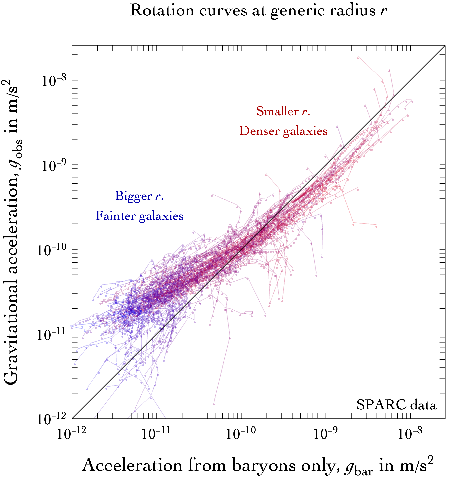
\includegraphics[width=0.45\textwidth]{figs/MONDgobsgbar} \qquad
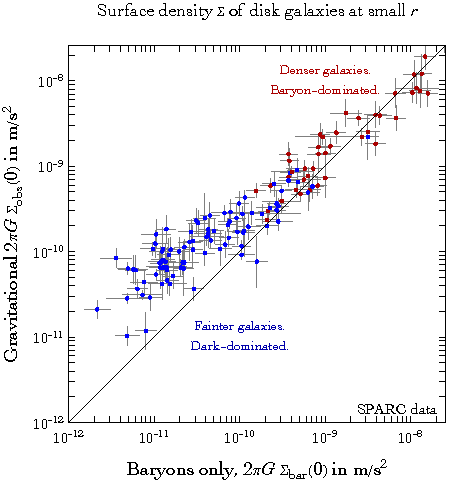
\includegraphics[width=0.45\textwidth]{figs/GalacticCentralDensity} 
\end{center}
\caption[MOND-motivated observations]{\em\label{fig:MONDdata2}
 {\bfseries Left}: correlation between the
centripetal acceleration $g_{\rm obs}=v^2/r$
observed in galactic rotation curves and
the gravitational acceleration $g_{\rm bar}$
computed from baryons only.
Galaxies with larger (smaller) surface brightness are in red (blue).
(\href{http://astroweb.cwru.edu/SPARC}{\color{black}SPARC galaxy data} from~\cite{gobsgbar}).
Weak lensing techniques try extending data down to $g_{\rm bar}\sim 10^{-15}\m/\s^2$
finding rough agreement with the MOND expectation $g_{\rm obs}\sim \sqrt{g_{\rm bar} a_*}$,
see \arxivref{2106.11677}{KiDS-1000} in~\cite{gobsgbar}.
{\bfseries Right}: correlation between the surface density $\Sigma(0)$ in galactic centers
as measured from baryons only and as measured from gravity.
(\href{http://astroweb.cwru.edu/SPARC}{\color{black}SPARC galaxy data} from~\cite{MONDr0}).}
\end{figure}



\subsection{Rotation curves at generic radii}\label{sec:MONDgenr}
The rotation curves contain more information than just that they are asymptotically flat.
The observations indicate that
{\em ``for any feature in the luminosity profile there is a corresponding feature in the rotation curve''},
known as Renzo's rule (from \arxivref{astro-ph/0311348}{Renzo Sancisi} in~\cite{DMvsa0}).
This is causally understood in baryon-dominated regions, 
but it is also observed in regions dominated by DM,
where it is unclear if correlations due to the formation history 
can explain this observation,
given that one would expect DM to have a roughly spherical and smooth density.

\smallskip

Motivated by MOND considerations, the full rotation curves have been studied,
in order to explore wether the radial gravitational accelerations $g_{\rm obs}(r)$, which have been measured in many systems,
correlate with the  acceleration $g_{\rm bar}(r)$ computed
based on the observations of baryons alone~\cite{gobsgbar}.
The results appear to be consistent with the MOND expectations:
the large spread between different rotation curves plotted in the middle-right panel in fig.\fig{rotationcurves}
collapses (within the significant uncertainties)
onto a common curve in fig.\fig{MONDdata2}a,
which also shows an indication of a possibly universal deviation from the $g_{\rm obs}=g_{\rm bar}$ equality, 
below the expected critical value of the acceleration.


The  near equality $g_{\rm obs}\approx g_{\rm bar}$ that is observed at large accelerations is a result of standard physics and is predicted both by MOND and DM;
the accelerations are large in the inner regions, which are dominated by baryonic matter and thus largely insensitive to DM.
The question on the other hand is, whether the tight correlation between $g_{\rm obs}$ and $g_{\rm bar}$ at lower accelerations
can arise in the DM context, 
namely, whether $\Lambda$CDM predicts similar enough formation histories for the various galaxies.


\subsection{Rotation velocities at small radii}
Baryonic matter, distributed on a thin galactic disk of surface density $\Sigma(r)$,
generates a Newton potential $\phi(r,z)$ according to the Poisson equation.
Rotation curves $v(r)$ on the galactic plane satisfy $v^2/r = - \partial\phi/\partial r|_{z=0}$.
By writing the potential $\phi$ as a Fourier integral over the basis functions $\phi_k=J_0(kr) e^{-k|z|}$,
one can show  that the surface density at the galactic center, $\Sigma(0)$, can be written as a weighted integral over rotation curves 
(\href{https://ui.adsabs.harvard.edu/abs/1963ApJ...138..385T/abstract}{\color{verdes}Toomre (1963)} in~\cite{MONDr0})
\beq
 2\pi G \Sigma(0) =  \int_{-\infty}^{+\infty} \frac{v^2(r)}{r}d\ln r.
\eeq
The above integral is dominated by the small $r$ region, so that the observed $\Sigma_{\rm obs}(0)$ is mostly determined by the measurements of the rotation curves in the smallest $r$ bins.
This can then be compared with the measurements of  the surface density close to the galactic center due to just the baryons, $\Sigma_{\rm bar}(0)$. 
After correcting for the deviations from the thin disk approximation,
one finds the results plotted in fig.\fig{MONDdata2}b.
Since these are effectively just a different way of combining 
the ``generic $r$'' results, discussed in section~\ref{sec:MONDgenr}, 
it is not surprising that the two lead to very similar conclusions (compare the two panels in fig.~\ref{fig:MONDdata2}). 
Galaxies with higher surface density again have baryon-dominated centers,
so that $\Sigma_{\rm obs}\approx \Sigma_{\rm bar}$,
while  in galaxies with lower surface density one finds $\Sigma_{\rm obs}> \Sigma_{\rm bar}$.
This indicates an extra dark component below a critical density $\Sigma_{\rm cr}$,
corresponding to the critical acceleration $2\pi G \Sigma_{\rm cr}$, roughly compatible with eq.\eq{aMOND}.
Once again, the deviation from the predictions of the baryonic Newtonian gravity
is compatible with a roughly-universal MONDian dynamics~\cite{MONDr0}.


\section{Can DM explain observed regularities in galaxies?}\index{DM problems!rotation curves regularities}
The observed regularities are intriguing and demand an explanation. 
Can they be understood in terms of DM, or do they signal a new universal phenomenon that is not due to DM?


\subsection{Flat rotation curves from DM?}
First, let us discuss the possible explanations within the DM framework. 
To understand better the problem, let us start from an over-simplified picture of a galaxy, taking
 baryonic matter of total mass ${\cal M}_b$ to be concentrated in the center, surrounded by an extended DM halo. For simplicity, let us assume that the DM halo at large enough radii has a density profile described by a simple power law
$\rho(r) \sim k_{\rm DM}/r^s$.
 At small radii, where baryonic mass dominates,  the rotation curves are given by $v = (G {\cal M}_b/r)^{1/2}$. At large radii the enclosed mass is dominated by the DM halo, and thus the rotation curves are given by 
 $v_\infty= \sqrt{k_{\rm DM} G} r^{1-s/2}$. 
 
 Flat rotation curves, $v_\infty= \sqrt{k_{\rm DM} G}$, are then obtained for $s=2$.
The transition from baryon-dominated to DM-dominated gravitational pull happens  
at the critical radius $r_{\rm cr}\sim ({\cal M}_b/k_{\rm DM})^{1/(3-s)}$ 
which encloses equal amounts of mass in baryonic matter and in DM.
At the critical radius the gravitational acceleration is $a_*\sim G{\cal M}_b/r_{\rm cr}^2$ which for $s=2$ gives 
$a_*\sim G k_{\rm DM}^2/{\cal M}_b $. 


Can the clustering of DM form structures that have the correct density profiles $\rho(r)$ to reproduce flat rotational curves?
In section \ref{sec:rho_from_analytic} we obtained the slope $s=2$ (see the discussion around eq.\eq{isothermalsphere}) from the iso-thermal sphere
approximation to DM clustering, while the more realistic
DM density profiles discussed in section \ref{sec:DMdistribution} and
table~\ref{tab:rhoprofiles} have scale-dependent slopes $s\sim 1-3$.
That is,  DM does tend to give ``flattish'' rotation curves, which agree well with data. A potential exception to this general agreement may be the measurements of gravitational potential around isolated galaxies using weak gravitational lensing~\cite{2406.09685}, which, if confirmed, would imply flat circular velocity curves that remain flat  
up to large distances, even up to $r\sim {\rm Mpc}$ and thus well beyond the expected virial radii of dark matter halos.


\subsection{Baryonic Tully-Fisher relation from DM?}\index{Tully-Fisher}\index{Rotation curves!Tully-Fisher}
\label{sec:Tully-Fisher}
The amount of dark and baryon matter  
changes from galaxy to galaxy,  while data indicates that $a_*$, 
which relates the two quantities via $a_* \sim G k_{\rm DM}^2/{\cal M}_b$ (see above), does not. 
To agree with the observations the DM halo mass (controlled by $k_{\rm DM}$) and the baryonic mass ${\cal M}_b$ for each galaxy therefore
need to be related according to ${\cal M}_b\propto k_{\rm DM}^2$.
This is equivalent to the baryonic Tully-Fisher relation $v_\infty \propto {\cal M}_b^{1/4}$~\cite{Tully-Fisher},
since the relation ${\cal M}_b\propto k_{\rm DM}^2$ implies that the flat rotation velocity, $v_\infty\sim\sqrt{k_{\rm DM}G}$, scales as ${\cal M}_b^{1/4}$. 

\smallskip



The challenge for DM is whether this non-trivial 
relation between two seemingly unrelated quantities can be explained dynamically through the process of  structure formation,
reproducing the common behaviour observed across a wide range of galaxies.
The answer to this question remains unclear~\cite{DMvsa0}. 
In the minimal $\Lambda$CDM model the galaxy formation histories do have a common element: 
normal matter falls into potential wells that were already formed by cold DM.
This does induce correlations between the distributions of DM and normal matter, though very naively one might have guessed that
it would have predicted a universal proportion between matter and DM. 
The Tully-Fisher relation instead demands  relatively less baryons in smaller galaxies.

\smallskip

The approximate analytic description of the gravitational collapse of collision-less DM, described in section~\ref{sec:rho_from_analytic}, 
predicts that the density 
of DM halos is 
controlled by the average cosmological DM density at the time the individual halo collapsed.
Neglecting the effects of cosmological evolution, this would then give DM halos that are characterised by a common density $\rho$.
Estimating the size $r$ of the galactic halo  from ${\cal M}\sim\rho r^3$, and using it in the velocity curve relation 
$v^2/r = G{\cal M}(r)/r^2$ then gives the estimate
$v_\infty  \sim [\sqrt{G\rho} {\cal M}]^{1/3}$. Taking $\rho$ to be common to all galaxies, this would then imply a scaling $v_\infty  \propto {\cal M}^{1/3}$, which clearly differs from
the Tully-Fisher one, $v_\infty \propto {\cal M}_b^{1/4}$.
Now, many crude approximations went into the above naive estimate. For one, the galaxies formed only relatively recently, at the redshift $z\sim 1$.
Taking into account that the inhomogeneities on different scales grow to become non-linear
at different times
(see, e.g.,\ section~\ref{sec:haloMf}) results in additional scale dependence, which tends to improve the agreement with observations.
Combining this dependence with the effects of baryon collapse, at least within a simple model, see, e.g., \arxivref{astro-ph/0107284}{Kaplinghat \& Turner (2001)} in~\cite{DMvsa0},
then gives a possible explanation of how a seemingly universal value of $a_*$  might arise dynamically, at least for larger galaxies, which have their central regions
dominated by baryons.



However, as argued by \arxivref{astro-ph/0110362}{Milgrom (2001)} in~\cite{DMvsa0},
the same $a_*$ is also seen in larger structures as well as in smaller galaxies, 
in which DM  dominates over baryons and accelerations are below $a_*$.
The regularities observed in galaxies seem to go well beyond the universality of DM halos.
They appear to involve baryons in a key way, even though baryons constitute only a small fraction of the total apparent mass of the halo, and are often concentrated in a disk that is an order of magnitude smaller in size than the DM halo. 
Since the fraction of baryons in stars vs.~gas seem to vary with galaxy size,  
this suggests that complex astrophysical phenomena are at play.
For example, baryonic matter gets partially ejected by astrophysical effects such as the gas heating and supernova explosions, where the effectiveness of these processes
depends on the escape velocity of the specific galaxy. 
This complexity renders the process of galaxy formation a challenging problem, and one that is not yet under good theoretical control. 
In the DM framework this complex astrophysics is presumably responsible for the observed regularities, with an important role played by
 the fact that smaller galaxies have a relatively lower baryon content
(examples are shown in the bottom row in fig.\fig{rotationcurves}).

Present numerical simulations and semi-analytic descriptions of galaxy formation within $\Lambda$CDM  do not yet
firmly differentiate between $v_\infty \propto {\cal M}_b^{1/4}$ and $v_\infty \propto {\cal M}_b^{1/3}$ scalings, and are also unable to definitively answer whether 
the simulated structures have low enough scatter in the seemingly universal laws to be compatible with the observations~\cite{DMvsa0}.
It may well be that both the flatness of the galactic rotation curves at large radii as well as the baryonic Tully-Fisher relation can be explained by a dynamical interplay between baryonic matter and DM during the process of galaxy formation. If this is indeed the case, then the observed regularities do not have any profound implications for fundamental physics. Instead, they would merely be a consequence of how normal matter and DM tend to cluster, with no deeper meaning.
The opposite is also possible; the fact that regularities have been observed despite the complex astrophysical environments is considered by some to 
point to a new fundamental law, the MONDian dynamics.

The number of measured rotation curves will increase by at least an order of magnitude by the end of the 2020s,
thanks to the ASKAP and the future SKA (Square Kilometre Array) telescopes. 
Time will tell, if future data will remain compatible with such universal laws.

\smallskip




\section{Can MOND explain the observed irregularities?}
\label{sec:MONDproblems}
\index{MOND!problems}
While MOND can elegantly explain the flat rotation curves and the baryonic Tully-Fisher relation, it does face difficulties in several other systems, in which the clear-cut MOND predictions appear to be violated. Some of these difficulties are, 
roughly ordered in the increasing degree of seriousness, as follows.\label{MONDproblems} 
\begin{itemize}
\item[i)] 

On sub-galactic scales, 
some {\bf globular clusters} of stars, such as Palomar 14 and NGC2419, appear not to follow the MOND predictions, even though they are located in the outermost regions of the Milky Way halo and therefore in low-acceleration conditions where MOND should apply~\cite{MONDfailuresandsuccesses}. 
The statistical significance of these observations is, however, under debate. 
For instance, it is possible that the globular clusters are on a highly eccentric orbit around the Milky Way, i.e.,~that they only `recently' entered the low-acceleration regime, and thus have not yet reached the limit of MOND dynamics.
Similarly, if the systematic uncertainties in the determination of the properties of the globular clusters were underestimated this could also ease the tension with MOND.
To settle the issue in favour of DM one would need to observe galaxies with an inner region dominated by normal matter,
an intermediate region in the MOND regime where rotation curves are instead Keplerian,
before reaching the outer DM-dominated region with flat rotation curves.

\item[ii)]
On super-galactic scales,
clusters of galaxies are among the first systems where the missing mass problem has been identified (see section~\ref{sec:evidencesmedi}).  
Since the accelerations within clusters are comparable to $a_*$, clusters of galaxies are also good testbeds for MOND. 
Over the years, a number of analyses found that {\bf MOND can only partially account for the missing mass in clusters}~\cite{MONDfailuresandsuccesses}. 
MOND predictions could in principle still agree with the data in the unlikely case that the observations have missed collision-less objects formed out of ordinary baryons 
(such as compact clouds) which would then have added up to the residual missing mass in the clusters. \\
The problem with MOND's predictions is exacerbated by the observations of the {\bf bullet cluster}, as well as by observations of the other collisions among galaxy clusters (section~\ref{sec:bullet}). These show that whatever substance is responsible for `dark matter', it
is spatially separated from visible matter. It is thus not simply tied to the distribution of normal matter, contrary to the MOND postulate. 
(In order to explain the bullet cluster result within MOND, some authors initially suggested adding 2 eV neutrinos, a possibility that is now excluded~\cite{MONDfailuresandsuccesses}.)




\item[iii)] Similarly to the bullet cluster, the {\bf DM-deficient galaxies} discussed in section~\ref{sec:DMdeficient} 
would in principle constitute an example in which normal matter does not follow MOND predictions. 
MOND theories predict a modification of gravity at large enough distances such that $a\circa{<} a_*$.
However, the challenge is finding DM-deficient galaxies in this regime.
 
\item[iv)] On cosmological scales,
the evidence for dark matter does not come merely from the galactic rotation curves, but most importantly from cosmological observations of the {\bf CMB and structure formation} (as discussed at length in section \ref{sec:evidencesmaxi}), i.e.,\ from several different length scales and accelerations~\cite{MONDcosmo}.\footnote{Regarding other possible tests on large scales it is worth mentioning that some researchers believe the observed cosmological
voids to be predicted to be much rarer within the standard cold DM cosmology, while their existence can instead be understood within MOND, supplemented, however, by some amount of DM in the form of 11\,eV sterile neutrinos~\cite{MONDfailuresandsuccesses}.} 
Note however that, according to \arxivref{2406.17930}{McGaugh et al.~(2024)}~\cite{JWSTearlygal}, 
observed galaxies formed faster than what Dark Matter predicts,
in agreement with MOND.



\end{itemize}
From a more conceptual point of view, note that the phenomenological MOND postulate, eq.\eq{MOND}, is not a consistent theory. 
Such an empirical law, for instance, violates momentum conservation:
the forces between two different masses are not equal and opposite, given that the lighter mass is subject to a bigger acceleration,
and therefore to a bigger MOND effect. Over the years, several different internally consistent
theories have been proposed, which lead to 
MOND-ian dynamics in particular limits. We will review theories motivated by MOND in section~\ref{sec:MONDth}.

These MOND-motivated theories can differ from the minimal phenomenological MOND postulate, 
predicting extra effects that can alleviate its difficulties, or lead to new ones.
For example, it has been argued that  the `DM deficient'
tension, mentioned in point iii) above, can be alleviated, at least in some systems,
by the  `{\em external field effect}' (EFE) acting on a small galaxy immersed in a massive host.
Indeed, in theories of modified gravity, external sources can contribute more to the
gravitational field than they do in Newtonian gravity.
\arxivref{2009.11525}{Chae et al.~(2020)}~in~\cite{MONDfailuresandsuccesses} claimed a statistical detection of the EFE
predicted by MOND theories.
Furthermore,  \arxivref{2210.13472}{Kroupa et al.~(2022)}~in \cite{MONDfailuresandsuccesses} interpreted some
asymmetric tidal tails of star clusters as EFE, and thus a challenge to Newtonian dynamics.

\medskip

The small-acceleration MOND proposal can be tested directly by measuring 
{\bf wide stellar binaries} away from external fields.
Accelerations in these systems are so low that the MONDian theories predict the orbital
velocities to receive an order unity enhancement compared to the
Newtonian dynamics. The DM framework instead predicts that there will be no deviations from Netwonian physics, given that only little amounts of DM mass would be involved.
Since the orbital periods of these systems are very long, the orbits are not fully reconstructed by observations.
However, about 10000 such systems are partially observed by {\sc Gaia}, allowing for statistical tests.
The interpretation of data requires modeling of the undetected companions and of the uncertain
eccentricity distributions of the wide binaries.
The present situation is confusing; while some authors that analysed the {\sc Gaia} data
claim that wide binaries agree with the Newtonian dynamics, and thus
exclude MONDian effects with up to $19\sigma$ significance (see \arxivref{2311.03436}{Banik et al.~(2023)} in~\cite{MONDwidebinaries}),
others instead claim a discovery of MONDian anomalies with a significance of up to $10\sigma$, and thus
an exclusion of Newtonian dynamics (see \arxivref{2305.04613}{Chae~(2023)} in~\cite{MONDwidebinaries}).
The main issue is that some wide binaries involve a third unseen object, that produces MONDian-like deviations from Newtonian gravity.


\smallskip


In the {\bf solar system}, the solar gravitational acceleration is about $10^4 a_*$ around Pluto's orbit,
and becomes smaller than $a_*$ at distance $r \approx 0.1\,{\rm lyr}$  from the Sun.
\arxivref{2403.09555}{Vokrouhlicky et al.~(2024)}~\cite{MONDfailuresandsuccesses} 
claim that simulations of comets and planetesimals around the Oort cloud
at distances $10^{-3}-1$ light years from the Sun 
prefer Newtonian dynamics over its MOND modification at $a\lesssim a_*$. 
Full MOND theories where this modification is screened by the EFE are not disfavoured.
However, \arxivref{2401.04796}{Desmond et al.~(2024)} in~\cite{MONDfailuresandsuccesses} claim that such MONDian theories predict a quadrupolar correction
to the Sun gravitational potential, which was not observed in the precise Cassini measurements of Saturn's orbit.







\section{Theories of Modified Newtonian dynamics}\label{sec:MONDth}
\index{MOND!theory}
All the theories discussed so far, most notably in chapters \ref{models} and \ref{BigDMtheories}, add to the Standard Model of particle physics
some extra field that, as far as observables in cosmology and astrophysics are concerned,
behaves as stable non-relativistic particles: Dark Matter.
Let us now turn our attention to the theories in which modifications of gravity account for at least some of the observations that are usually interpreted in terms of DM~\cite{MONDth}. 
 As we will see, it is  hard to  bypass cold DM or something  similar to it, and match all observations. 


As discussed around eq.\eq{MOND}, 
galactic rotation curves motivate 
a specific modification of Newtonian gravity that kicks in on galactic scales --- MOND~\cite{MOND}.
That is, flat rotation curves compatible with observations are obtained, if at low accelerations $a \ll a_* \approx H_0$,  the equation of motion for a test particle
is modified from its form given by Newtonian gravity, $a = GM/r^2$, to a  MONDian form,
 $a^2/a_* = GM/r^2$ (with $a_*$ given in eq.\eq{aMOND}). 


\smallskip
This change can  be accomplished either by modifying inertia or gravity. 
A modification of inertia of the right magnitude could, for instance, occur by having the existence of a cosmological horizon affect the inertia of bodies through a Hubble-scale Casimir-effect (see, e.g.,\ \arxivref{astro-ph/9805346}{Milgrom (1999)}  in~\cite{MONDth}).
In effect, one postulates $\sim H_0$ as the minimal acceleration, based on the observation that, at low accelerations, the horizon of 
the coordinates for a uniformly accelerating reference frame in flat spacetime (Rindler coordinates) becomes comparable to
the cosmological horizon (see, e.g.,\  \arxivref{1004.3303}{McCulloch (2010)} in~\cite{MONDth}). 
Developing the heuristic arguments for $a_* \sim H_0$ into a full theory has, however, proved to be quite challenging.

A related highly non-standard proposal is that gravity might be an emergent phenomenon, related to entanglement entropy (`{\bf emergent gravity}'~\cite{emergentgravity}), 
and that this could explain Newtonian gravity together with a MOND-like modification 
below a critical acceleration that is comparable to the current acceleration of the Universe. 
It is not yet clear whether this idea can reproduce relativistic gravity
(tested in environments such as the solar system, dwarf galaxies and galaxy clusters~\cite{testsofEG})
and the observed cosmological CMB anisotropies.
A different non-standard  proposal assumes that gravity behaves classically up to stochastic corrections that might 
mimic a minimal accelerations similar to what postulated by MOND~\cite{Oppenheim}.

\medskip

Modifications of gravity, more precisely the gravitational acceleration $g$, have been proposed in several tentative realizations using field theories. These introduce extra fields, very much like in DM theories. 
The first step in this direction was the construction of a non-relativistic field theory for MOND 
by \href{https://doi.org/10.1086/162570}{Bekenstein and Milgrom (1984)} in \cite{MONDth}, who
modified the Poisson equation for the non-relativistic Newton potential $\phi$
at small gravitational fields, $ x \equiv (\vec\nabla \phi)^2/ a_*^2 \ll 1$, by assuming a non-relativistic Lagrangian density of the form
\beq 
-\Lag_{\rm MOND}^{\rm non~rel}= \frac{a_*^2 J(x)}{8\pi \tilde G } 
 + \phi \rho,\qquad
 \hbox{implying}\qquad
\vec{\nabla}\cdot \left[J'\left(x\right) \vec\nabla \phi\right] = 4\pi \tilde G \rho,
\eeq
where $\rho$  is the baryonic mass density and $J(x)$ is some function.
Newtonian gravity is obtained for the usual quadratic action, $J(x)=x$ and $\tilde G = G$.
MOND is obtained if $J' (x)\simeq \sqrt{x}$ in the limit $x\ll 1$, corresponding to  
$J(x) \simeq \frac23 x^{3/2}$.
In this limit a point mass $M$ sources $\phi \simeq \sqrt{GM a_0}\ln r$ and thereby an acceleration 
\beq \vec a=-\vec \nabla \phi =- \sqrt{\tilde GM a_*}\vec r/r^2\qquad\hbox{at} 
\qquad r \gg r_*\equiv \sqrt{\tilde G M/a_*},\eeq
resulting in the desired $v(r)$ dependence of galactic rotation curves, eq.\eq{MOND}. 
The above theory extends the MOND postulate beyond spherical or cylindrical symmetry,
and respects momentum conservation, since its action is invariant under translations.
However, it is  neither Galilean nor Lorentz invariant: 
gravity is corrected in a way that is vaguely analogous to how a dielectric modifies equations of  electromagnetism, 
so that the physics depends on the absolute acceleration with respect to the special `rest' frame.
This gives the `{\em external field effect}', already anticipated in section~\ref{sec:MONDproblems}:
forces within a system that is embedded in a bigger external system (such as a galaxy in a cluster of galaxies)
also depend on the gravitational acceleration $\vec{g}_{\rm ext}$ of the latter.
In contrast, Newtonian and Einstein gravity give rise to tidal forces only, 
related to spatial gradients of $\vec{g}_{\rm ext}$, and thus respect the strong equivalence principle.

\smallskip

Since theories of gravity are strongly constrained by general covariance, 
it is convenient to also consider another class of MOND theories: those that can avoid modifying the action for the Newtonian potential $\phi$.
Keeping its usual action, this can be obtained by
adding a scalar $\mond$ that kinetically mixes with $\phi$, giving the Lagrangian 
\beq\label{eq:MONDnonrel}
 -\Lag _{\rm MOND}^{\rm non~rel} 
= \frac{1}{8\pi \tilde G}\left[ [\vec\nabla (\phi -\mond)]^2 +  a_*^2 J(y) \right] + \phi \rho,\qquad
y \equiv  \frac{|\vec\nabla \mond|^2}{a_*^2}.\eeq
There are various choices for function $J$, which smoothly interpolate between the Newtonian and MOND limits.
To avoid conflicts with precision solar-system measurements (such as the precession of orbits), 
one needs a function $J$ that quickly reduces to Newtonian gravity in its regime of validity,
such that MOND effects are strongly suppressed
(see, e.g.,\ \arxivref{0903.3602}{Skordis (2009)} in~\cite{MONDth}).


\subsection{MOND as tensor-vector-scalar gravity}
The formulation of MOND in eq.~\eqref{eq:MONDnonrel} paves the way for the next step; to go beyond the small-velocity and weak-field limits,
and find a MONDian extension of general relativity.
The best known extension of this sort is the TeVeS construction by \arxivref{astro-ph/0403694}{Bekenstein (2004)} in~\cite{MONDth}.
In TeVeS, the Newtonian potential $\phi$ is, as in the usual general relativity,  given by the $g_{00}$ component of the  Einstein metric $g_{\mu\nu}$, 
$g_{00} = 1+2\phi$, while the scalar $\mond (\vec x)$ becomes a shift-symmetric Lorentz scalar $\mond (x_\mu)$.
In order to obtain from a covariant action the peculiar MONDian action with the unusual spatial gradients,
an extra four vector $U_\mu$ with time-like unit norm, $U_\mu U^\mu=1$,  is introduced
(thus the TeVeS acronym, which stands for the Tensor-Vector-Scalar gravitational field content).
The main role of $U_\mu$ is to be able to induce the desired mixing of
the scalar $\mond$ with the Newtonian gravitational potential $\phi$
(for the details see below).
The field $U_\mu(x)$ has a non-vanishing vacuum expectation value $\med{U_\mu}$  along the time direction, which then
selects a special frame and
breaks the strong equivalence principle.\footnote{In the $\Lambda$CDM framework the cosmological evolution instead selects a special frame, in which the Dark Matter and ordinary matter are at rest, on average.}



\smallskip

In this initial version of TeVeS, ordinary SM fields couple to a modified metric $\tilde g_{\mu\nu}$, which is a function of
$g_{\mu\nu}$, $U_\mu$, and $\mond$. 
Consequently, these theories predicted that the electromagnetic and gravitational waves would have different  speeds of propagation. 
This prediction was contradicted by the simultaneous detection of gravitational waves from a neutron star
merger (GW170817) and its electromagnetic counterpart in the form of a gamma-ray burst.
The close arrival times of the two signals limited
the allowed difference in the speeds of photons and gravitons to be less than about one part in $10^{15}$, 
excluding TeVeS and similar theories of MOND~\cite{GWandMOND}.


\smallskip

Putative MOND-ian extensions also face challenges with cosmological measurements. 
The main challenge is how to mimic the cosmological imprints that are a result of a two-component fluid in the standard $\Lambda$CDM cosmology: the noninteracting DM fluid and the interacting plasma composed of normal matter and photons. 
As discussed in detail in section~\ref{sec:linear:inhom},
the two components behave differently and thus also evolve differently. The fluctuations in DM evolve under the influence of gravity, while the fluctuations in the baryon-photon fluid oscillate as sound waves. 
After recombination, the baryons decouple from photons and fall into the growing gravitational potential wells due to DM. 
This process erases most of the signatures of the sound waves, and  explains why there are ${\mathcal O}(1)$ oscillations seen in the CMB (section~\ref{sec:CMB}), 
and much smaller ones in the distribution of galaxies,  ${\mathcal O}\big(\Omega_b^2/\Omega_{\rm DM}^2\big)\sim 0.04$.
The MOND-ian theories need to achieve this suppression of acoustic fluctuations~\cite{MONDcosmo} without introducing a non-interacting fluid, such as a gas of cold DM particles.
It has been suggested that a MOND cosmology that contains sterile neutrinos (which are too hot to be a cold DM) might agree with the CMB data,
although structure formation might be problematic~\cite{MONDcosmo}.

\medskip


Skordis and Zlosnik proposed a relativistic theory of MOND that is claimed to solve the above problems (\arxivref{1905.09465}{Skordis and Zlosnik (2019)} and \arxivref{2007.00082}{(2020)} in~\cite{MONDth}).
The Lagrangian of the theory contains the SM fields coupled to $g_{\mu\nu}$, in the same way as in general relativity, and a modified
gravitational sector 
\beq \Lag_{\rm MOND}^{\rm TeVeS-SZ} = \frac{1}{16\pi \tilde G}\left[
R - \lambda(U_\mu U^\mu+1)-
 \frac{K_B}{2} F^{\mu\nu}F_{\mu\nu} + 
  (2-K_B)  [2 J^\mu (\nabla_\mu\mond)- Y]- F(Q,Y)\right]+ \Lag_{\rm SM},
\eeq
where $\lambda$ is a Lagrange multiplier that fixes $U^\mu$ to be a unit time-like vector,
with $F_{\mu\nu} \equiv 2(\nabla_\mu U_\nu - \nabla_\nu U_\mu)$,
$J^\mu\equiv U^\alpha \nabla_\alpha U^\mu$, while
$F$ is some function of
\beq 
Y\equiv(g^{\mu\nu} +U^\mu U^\nu)(\nabla_\mu\mond)(\nabla_\nu\mond)
\qquad\hbox{and}\qquad Q\equiv U^\mu \nabla_\mu \mond.
\eeq
To see how the theory works, let us specialize to the cases of dynamics on the galactic scale and to cosmology:
\begin{itemize}
\item[$\triangleright$]  In the non-relativistic limit 
$Y$ reduces to $(\vec{\nabla}\mond)^2$, 
and $J^\mu (\nabla_\mu \mond)$ to $(\vec\nabla\phi)\cdot(\vec\nabla\mond)$.
The theory then reduces to the desired form in eq.\eq{MONDnonrel}
plus an additional quadratic  ``mass term'' for the Newton potential $\phi$.
This undesired term  is proportional to $\dot\mond$, and must be smaller than $\sim 1/{\rm Mpc} \sim 10^{-30}\eV$ in order to reproduce the galactic
rotation curves {\em \` a la} MOND.
The critical acceleration $a_* $ depends on 
the scalar vacuum expectation values, and  $a_* \sim H_0$ is not a generic outcome.


\item[$\triangleright$]
The cosmological time evolution of $\mond$ allows the scalar $\mond$ to play the role of DM in cosmology.
Let us consider the homogenous limit where $\mond$ depends only on time.
This corresponds to $Y=0$ and $Q = \dot\mond$, so that the scalar Lagrangian
reduces to $\Lag = - F(Q,0)/16\pi\tilde G$.
Assuming a kinetic energy for $\mond$ minimal at $\dot\mond\neq 0$ gives a kinetic analogue of the Higgs phase,
known as the `ghost condensation' or the `$K$-essence'.
The classical equation of motion, $\ddot\mond F'' + 3 H F'=0$, is solved by $ F' \propto 1/a^3$.
Let us assume that $F$ can  be approximated close to its minimum as a quadratic function of $\dot\mond^2$,
$F \simeq F_0 + F_2 (\dot\mond^2 - \dot\mond_0^2)^2$, where $F_0, F_2$ and $\dot\theta_0$ are constants~\cite{Kessence}.
The resulting approximate solution for $\theta$ is thus $\dot\mond \simeq \dot\mond_0$.
The energy density of the field $F$, given by $\rho = (\dot\mond F' - F)/8\pi\tilde{G}$,
then contains two terms: the first scales as $1/a^3$ (like matter), the second is constant (like vacuum energy).
In this limit, the perturbations of the system have a small sound speed.
An appropriate function $F$ away from the minimum is needed during the cosmological evolution.

\item[$\triangleright$] 
Linear fluctuations in cosmology behave as  they would in normal general relativity in the presence of cold dark matter, but with an additional non-standard
pressure that can be small enough~\cite{MONDth}. 
In this way, the theory can reproduce the CMB temperature spectrum, an otherwise long-standing problem for the MOND idea (see the discussion on page \pageref{MONDproblems}).
 In the nonlinear regime it is expected that the two theories differ, but the observable consequences are yet to be explored. 

\item[$\triangleright$] 
The introduction of a purely anti-symmetric $F_{\mu\nu}$, means that
the waves in the symmetric $g_{\mu\nu}$ tensor can behave exactly as they do in the Einstein theory:
expanding over a Minkowski background
the photon and graviton speeds therefore remain equal~\cite{MONDth}.

\end{itemize}
The above set-up does not solve all the observational problems; open issues remain.
For instance, it is not clear how the theory can explain the behaviour of the bullet cluster 
and of ordinary galaxy clusters, analogously to what discussed in sec.~\ref{sec:MONDproblems}~\cite{MONDfailuresandsuccesses}.
The CMB polarization spectra might be affected by $U_\mu$. Furthermore, the 
action for $U_\mu$ seems not to be gauge invariant, endangering the quantum consistency of the theory~\cite{MONDth}.


\medskip

\subsection{MOND as a superfluid Dark Matter}\label{superfluidDM}
\index{MOND!as superfluid DM}\index{Super-fluid DM}
As we saw above, tentative theories of MOND, when written in the universal language of
Quantum Field Theory, employ new fields, similarly to theories of Dark Matter.
One can similarly try to devise a theory of Dark Matter that acquires a MONDian behavior on galactic scales,
while behaving as matter in cosmology.
A  possibility in this direction is that the scalar field $\mond$ has nothing to do with gravity,
and mediates the desired MOND force because  it couples to the matter density similarly to gravity, as $\mond \rho$.
To match the MONDian dynamics, its non-relativistic Lagrangian must contain the unusual $|\vec{\nabla}\mond|^{3/2}$ term.

A possible justification for such a term could  be DM super-fluidity~\cite{DMsuperfluid}.
Going against the original intention of MOND, let us assume the existence of a relativistic complex scalar field $\varphi$,
which gives rise to the usual DM in cosmology.
As discussed in section~\ref{LightBosonDM}, DM occupation numbers become larger than unity
in galaxies, if the DM mass is $M\lesssim \eV$.
In this regime a phenomenon familiar from condensed-matter can take place: 
DM can form a Bose-Einstein condensate (as in section~\ref{LightBosonDM}), and become super-fluid.
This phenomenon occurs if the phonon fluctuations of the DM condensate are ultra-light.
This composite degree of freedom can play the role of $\mond$, giving MONDian dynamics on galactic scales.

Indeed, the ultra-light phonon field $\theta$ can be understood in quantum field theory as the Goldstone boson of the global U(1) symmetry describing the conservation of the $\varphi$ particle number, which
gets spontaneously broken by the finite-density condensate $\langle\varphi\rangle=v \,e^{i \mu t}$, where $\mu$ is a chemical potential.
Parameterizing the relativistic field as 
$ \varphi (x)= [v+h(x)] e^{i[\mu t + \mond(x)]}$
and expanding its Lagrangian in the non-relativistic limit,
the Goldstone boson $\mond$ acquires an effective Lagrangian of the desired MOND type, 
if the initial relativistic Lagrangian is
\beq 
\Lag_{\rm MOND}^{\hbox{\scriptsize super-fluid}} = |\partial_\mu \varphi|^2 - M^2 |\varphi|^2 - V(\varphi) +\Lag_{\rm SM}, 
\eeq
with the unusual repulsive potential $V \propto c |\varphi|^6$~\cite{DMsuperfluid}.
The effective action for the light phonon $\mond$  depends only on the combination
$X\equiv \mu + \dot{\mond} - (\vec\nabla\mond)^2/2M$, due to the Galilean invariance of the theory (i.e., due to the non-relativistic remnant of the full Lorentz invariance). 
The special form of the potential gives rise to the $X^{3/2}$ power needed to obtain MOND.
However, MOND needs $c<0$, which leads to instabilities.
More complicated actions separate the $X=0$ vacuum from such instabilities, and alternative models assume a non-minimal kinetic term. 
However issues such as super-luminality remain in the theories, questioning their fundamental viability~\cite{DMsuperfluid}. 
Proceeding anyway,
the phonon $\mond$ mediates a MOND-like force on galactic distances, if one
adds to $\Lag_{\rm SM}$ an additional U(1)-breaking interaction of the phonon to matter of the form $\theta\rho$.
A very small coupling is needed to obtain the desired value of $a_* \sim H_0$. 
The end result is something akin to the Landau two-fluid model:
a fraction of DM remains in the form of particles, while a fraction of it forms a superfluid with a cored galactic profile, which leads to the MONDian dynamics.
In this context MOND is an outcome of special properties of the DM system, rather than an alternative to DM.




There are differences between the above set-up and the simple MOND postulate. 
For instance, it is reasonable to assume that, unlike gravity, phonons interact with baryon but not with photons. 
\arxivref{2303.08560}{T. Mistele et al.~(2023)} in~\cite{DMsuperfluid} then argue that this difference makes the super-fluid DM incompatible with the weak lensing data.

\section{Conformal gravity}\label{ConformalGravity}
\index{Conformal gravity}
Finally, we summarise a different attempt at interpreting galactic rotation curves as modified gravity, without DM.
In general, pure Einstein gravity, with the action $S_{\rm E} = \int d^4x \sqrt{|\det g|}[-\bar{M}_{\rm Pl}^2 R/2 - V]$, 
might be the low-energy limit of a deeper theory.
An interesting possibility for the latter is the so called {\em conformal gravity} which has as the action
\beq 
S_{\rm C} =\int d^4x \sqrt{|\det g|} \frac{R^2/3 - R_{\mu\nu}^2}{f_2^2}.
\eeq
$S_{\rm C}$ is non-trivially invariant under a Weyl rescaling of the metric, $g_{\mu\nu}(x)\to \Omega^2(x) g_{\mu\nu}(x)$ for arbitrary $\Omega(x)$.
For example, $f_2$ is a dimension-less constant signalling scale invariance and renormalizability.
Classical equations of conformal gravity admit a spherical  solution~\cite{ConformalGravity}
\beq \label{eq:krmetric}
ds^2 = f(r)\, dt^2 - \frac{dr^2}{f(r)} - r^2 (d\theta^2 +\sin^2 \theta\, d\varphi^2),\qquad f(r) = \sqrt{1-6 GM k} - \frac{2GM}{r} + k r  - \frac{V}{3\bar{M}_{\rm Pl}^2} r^2,
\eeq
where $V$, $GM$ and $k$ are three constants of integration.
One of them, $M$ corresponds to the local mass in the solutions to Einstein gravity.
The two additional integration constants $k$ and $V$
arise because the conformal gravity action leads to equations of motion that contain 4 powers of derivatives
and correspond to long-range effects.
So they are expected to be the same in all different galaxies.
In particular, in the $k=0$ limit, eq.\eq{krmetric} reduces to the Schwarzschild-de Sitter vacuum solution of Einstein gravity with a vacuum energy $V$.
In the small-$r$ limit eq.\eq{krmetric} reduces to Einstein gravity and to the Newton potential,
in agreement with observations (for example in the solar system).

In the Newtonian limit, the extra $kr$ term corresponds to a gravitational potential growing with distance, and thereby to a constant force.
A constant force does not make galactic rotation curves flat (a force $F \propto 1/r$ would be needed).
Nevertheless, it has been proposed that the observed galactic rotation curves can be reproduced by the appropriate form of $f(r)$, 
without the need for DM,
by fitting different values of $M$ for each galaxy,
while $k$ and $V$ are assumed to be universal~\cite{ConformalGravity}.
%This is possible because $M,k,V$ are integration constants; for example $V$ is not a universal vacuum energy.

This proposal faces several theoretical issues~\cite{ConformalGravity}:
$i)$ 4-derivative equations of motion imply the classical Ostrogradsky instability and a ghost state at quantum level.
$ii)$ A Weyl transformation and a redefinition of $r$ allows to remove the $kr$ term, bringing back eq.\eq{krmetric} to the Schwarzschild-de Sitter form.
This issue is debated by \arxivref{2105.14679}{Mannheim (2021)} in~\cite{ConformalGravity}.
$iii)$ The conformal symmetry is broken at microscopic level, for example by the quantum running of SM couplings and by the Higgs mass.
$iv)$ It's unclear how such a proposal could give a DM-like effect in cosmological CMB and large scale structure data,
and the associated gravitational lensing on cosmological scales.
See~\cite{CottonGravity} for a related attempt, not based on an action.

This underscores the many challenges faced by the efforts of  trying to match some observations by only modifying gravity, 
while not introducing new degrees of freedom (such at DM).




